\subsection{Game Management System Interface}
\label{app:llms_screenshots}

In this appendix, we present the main features of our game management system through a series of screenshots. The system facilitates data collection and analysis from the games described in \S\ref{sec:game_families}, offering a user-friendly and customizable interface.

The main interface of the system (Figure~\ref{fig:main_screen}) provides three primary options: starting a new data collection, resuming a previously interrupted collection, and analyzing results from past experiments. When initiating a new data collection, users first select the game family and the participating LLMs (Figure~\ref{fig:new_exp_1}), followed by defining the set of configurations to be executed (Figure~\ref{fig:new_exp_2}). 

Once the data collection is complete, users can move to the analysis phase. The data analysis module starts with selecting the data to be analyzed (Figure~\ref{fig:analyze}). After selecting the relevant data, users can use the parameter impact viewer (Figure~\ref{fig:analyze_results}) to visualize how game parameters influence various metrics (see \S\ref{par:statistical_analysis}). Additionally, the system provides a statistics table (Figure~\ref{fig:statistics}) that summarizes key characteristics of the collected data.

The system does not require any specialized hardware: data collection and analysis can be performed efficiently using a single CPU.

\begin{figure}[H]
\centering
\fbox{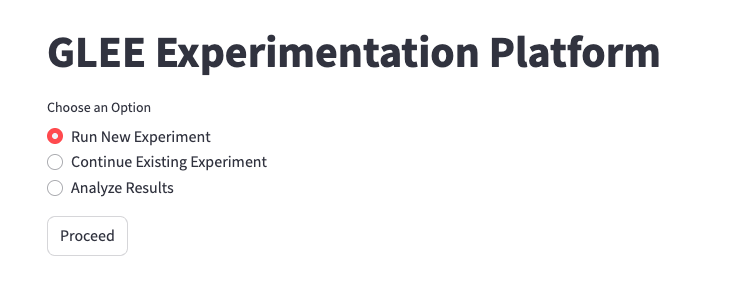
\includegraphics[width=0.75\textwidth,height=\textheight,keepaspectratio]{screenshots/llms_screenshots/main_screen.png}}
\caption{Main interface: Start a new data collection, resume a previous one, or analyze results from past experiments.}
\label{fig:main_screen}
\end{figure}

\begin{figure}[H]
\centering
\fbox{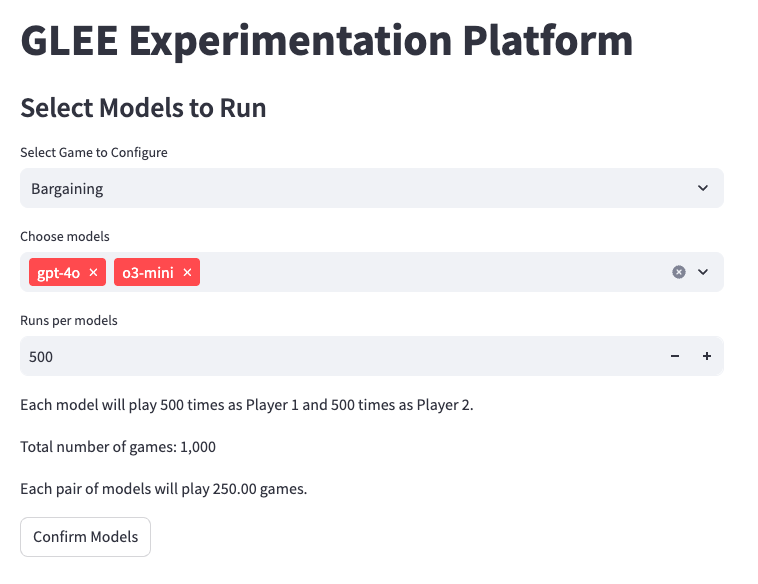
\includegraphics[width=0.75\textwidth,height=\textheight,keepaspectratio]{screenshots/llms_screenshots/new_exp_1.png}}
\caption{New data collection: Selecting game family and LLMs.}
\label{fig:new_exp_1}
\end{figure}

\begin{figure}[H]
\centering
\fbox{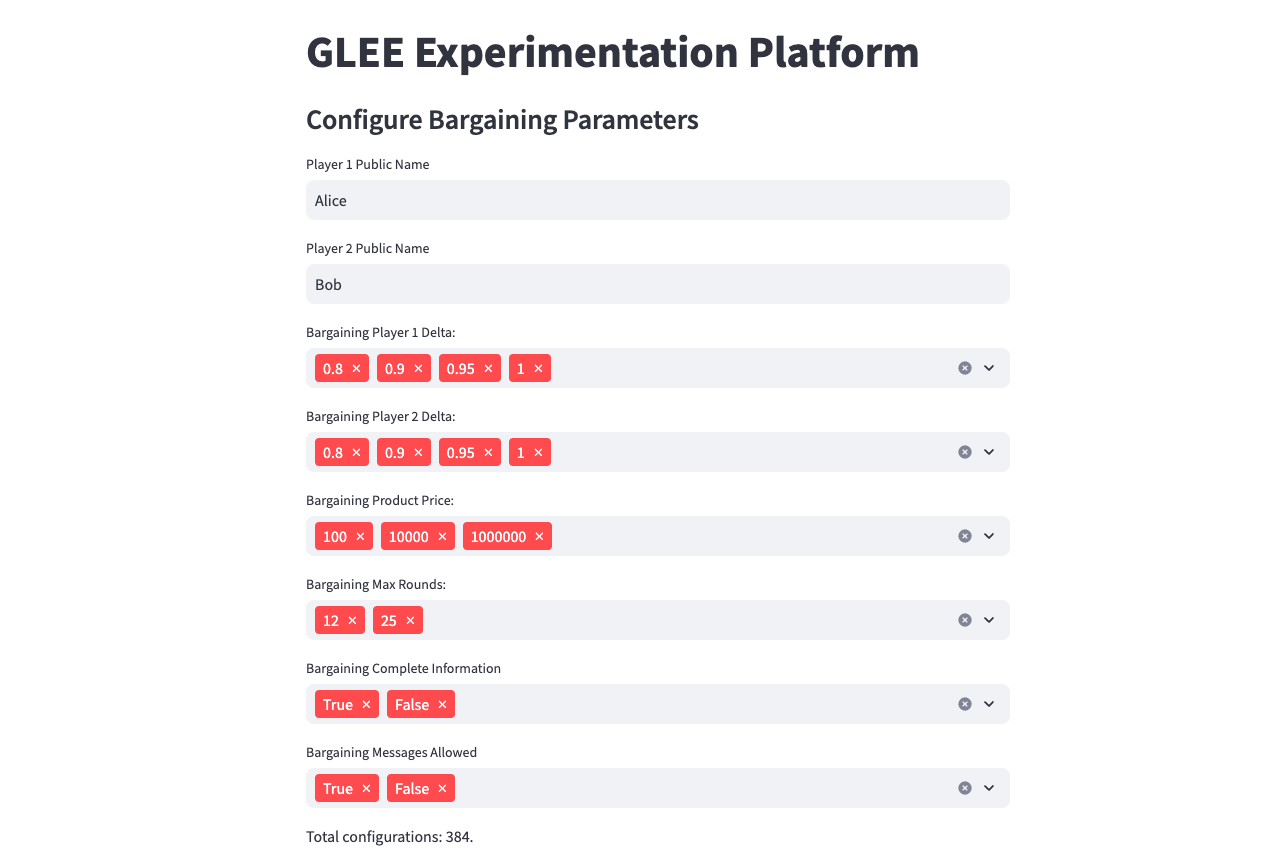
\includegraphics[width=0.75\textwidth,height=\textheight,keepaspectratio]{screenshots/llms_screenshots/new_exp_2.png}}
\caption{New data collection: Setting up configurations.}
\label{fig:new_exp_2}
\end{figure}

\begin{figure}[H]
\centering
\fbox{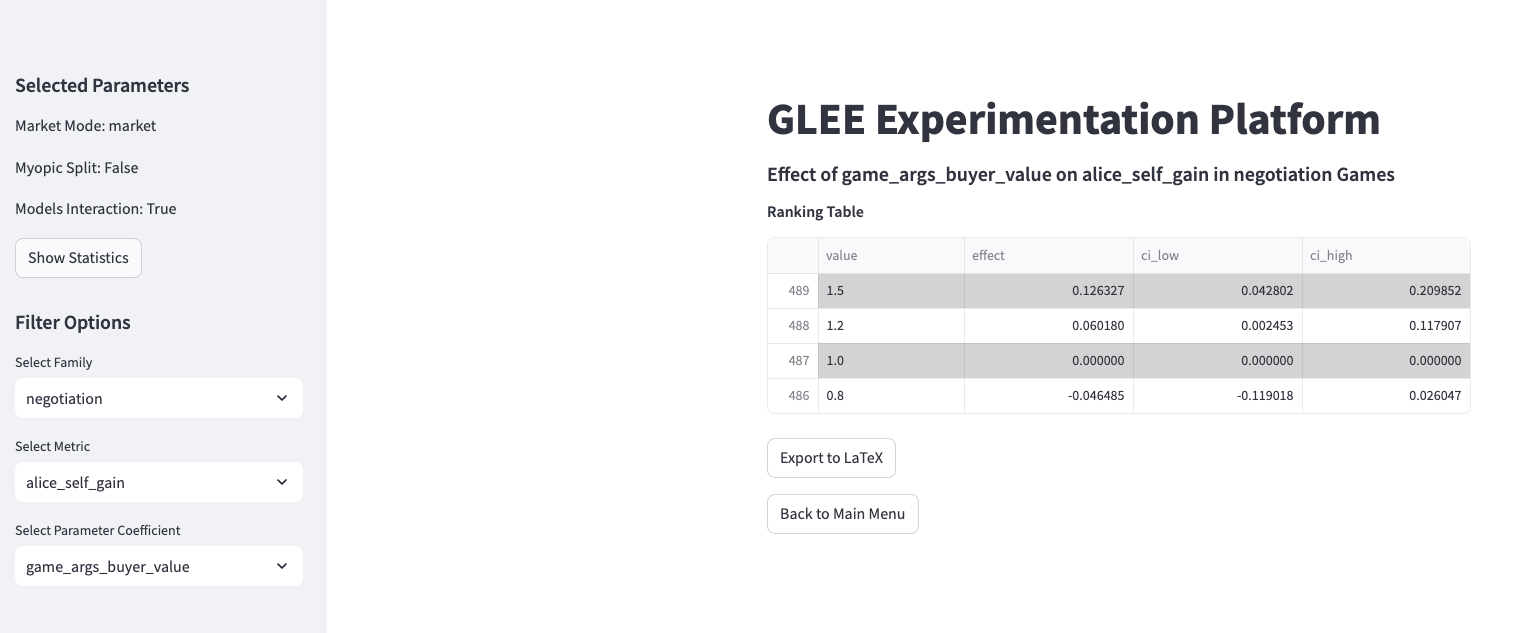
\includegraphics[width=0.75\textwidth,height=\textheight,keepaspectratio]{screenshots/llms_screenshots/analyze.png}}
\caption{Data analysis: Selecting datasets for analysis.}
\label{fig:analyze}
\end{figure}

\begin{figure}[H]
\centering
\fbox{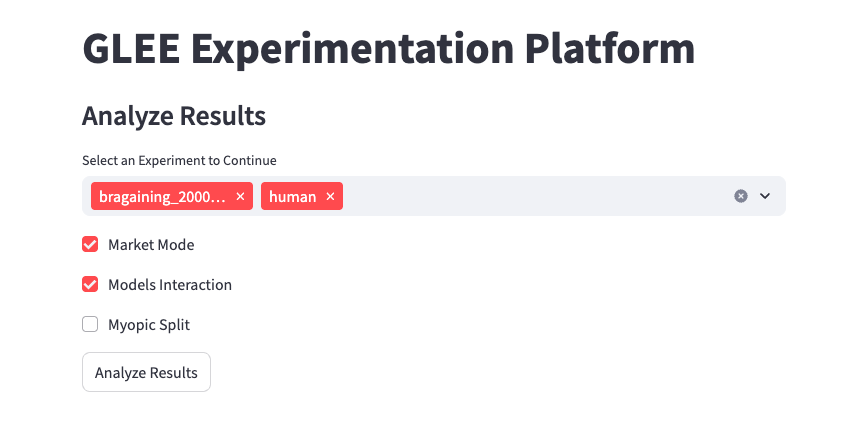
\includegraphics[width=0.75\textwidth,height=\textheight,keepaspectratio]{screenshots/llms_screenshots/analyze_results.png}}
\caption{Data analysis: Visualizing the impact of game parameters on various metrics.}
\label{fig:analyze_results}
\end{figure}

\begin{figure}[H]
\centering
\fbox{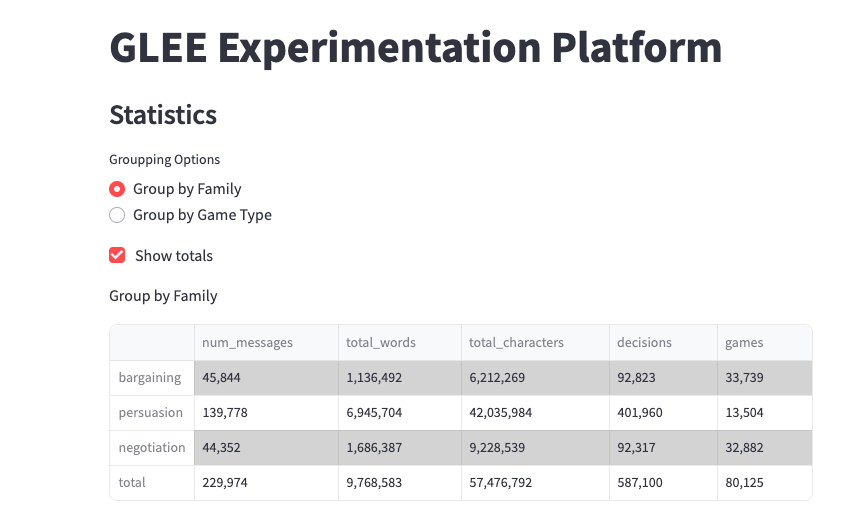
\includegraphics[width=0.75\textwidth,height=\textheight,keepaspectratio]{screenshots/llms_screenshots/statistics.png}}
\caption{Data analysis: Statistics table summarizing key characteristics of the collected data.}
\label{fig:statistics}
\end{figure}



\subsection{Conversation Structures}
\label{app:system}
% Define Alice's colors
\newcommand{\aliceSystem}[1]{\textcolor{red}{#1}}
\newcommand{\alicePrompt}[1]{\textcolor{purple}{#1}}
\newcommand{\aliceMessage}[1]{\textcolor{magenta}{#1}}

% Define Bob's colors
\newcommand{\bobSystem}[1]{\textcolor{blue}{#1}}
\newcommand{\bobPrompt}[1]{\textcolor{teal}{#1}}
\newcommand{\bobMessage}[1]{\textcolor{cyan}{#1}}

In this appendix, we present an example of the conversation structures with the language models used for data collection in \textit{GLEE}. The example is from a bargaining game, but the system's operating principle is the same in negotiation and persuasion games as well.

The prompts are divided into two types: (1) instructions and guidelines sent to the language model as a system message, and (2) game management messages sent to the language model as a user message. The language model performed its action, which was documented in the prompt as an assistant message. The system message begins with precise game instructions, which are constructed at the start of the game using the parameters that define the configuration. This is followed by a guideline specifying the format in which the LLM is required to respond. Each time the language model is required to make a decision (of any type), the language model receives a message containing all the information that has accumulated since its previous turn. This information appears as a system message and sometimes includes text written by the language model that played the second player.

It was possible to alter the prompt that introduces the game, explore different variations, and allow the language models to play different personas. While this could impact the behavior of the language models, budget limitations would have required us to collect less data from each configuration. Therefore, we chose to keep the prompt fixed rather than further defining the language model's setup. However, the system allows easy prompt customization to support future research.

Throughout the appendix, the \aliceSystem{system prompt (or parts of it) that Alice received are highlighted in red}. \alicePrompt{Game management messages Alice received are shown in purple}, and \aliceMessage{her response is shown in magenta}. The \bobSystem{system prompt that Bob received is highlighted in blue}. \bobPrompt{Game management messages Bob received are shown in teal}, and \bobMessage{his response is shown in cyan.}


\noindent\hrulefill

Instructions to Alice:

\aliceSystem{Let's play a game.
In this game, there are two players. You are playing as Alice. You and Bob need to divide 1,000\$ between you.
In each round of the game, one of the players will make a proposal for division and can describe their proposal in a few words. The other player will decide whether to accept the offer and finish the game, or to proceed to the next round, in which they will be the one making the proposal.
We will relay messages between you and Bob.
Beware of inflation! With each passing round, the money is worth 0\% less for you. For Bob, the money is worth 10\% less. You have 10 rounds to divide the money, or both of you will get nothing!}

Instructions to Bob:

\bobSystem{Let's play a game.
In this game, there are two players. You are playing as Bob.
You and Alice need to divide 1,000\$ between you.
In each round of the game, one of the players will make a proposal for division and can describe their proposal in a few words. The other player will decide whether to accept the offer and finish the game, or to proceed to the next round, in which they will be the one making the proposal.
We will relay messages between you and Alice.
Beware of inflation! With each passing round, the money is worth 10\% less for you. For Alice, the money is worth 0\% less. You have 10 rounds to divide the money, or both of you will get nothing!}

\noindent\hrulefill

Alice turn.

Alice got this message from the system:

\alicePrompt{'Round 1\\
Send your offer to divide \$1,000 and a message to Bob.'}

Alice guideline:

\aliceSystem{Send your offer to divide 1,000\$ and the message you attached in the JSON format: \\
\{"alice\_gain": The part that you will receive in your offer,\\
"bob\_gain": The part that Bob will receive in your offer,\\
"message": The message you pass to Bob\}}

Alice's response:

\aliceMessage{```json
\{"alice\_gain": 900, "bob\_gain": 100,\\ "message": "Let's start fair. I'll take the bigger share, but you get something too."\}
```
}

\noindent\hrulefill

Bob turn.

Bob got this message from the system:

\bobPrompt{Round 1\\
Alice's offer:\\
\# Alice's message: Let's start fair. I'll take the bigger share, but you get something too.\\
\# Bob gain: 100\\
\# Alice gain: 900\\
Do you accept this offer?}

Bob guideline:

\bobSystem{Answer with \{"decision": "accept"\} or \{"decision": "reject"\}}


Bob's response:

\bobMessage{```json
\{"decision": "reject"\}
```}


\noindent\hrulefill

Bob turn.

Bob got this message from the system:

\bobPrompt{You have chosen to reject Alice's offer from round 1.\\
Round 2\\
Send your offer to divide \$1,000 and a message to Alice.}

Bob guideline:

\bobSystem{Send your offer to divide 1,000\$ and the message you attached in the JSON format:\\
\{"bob\_gain": The part that you will receive in your offer,\\
"alice\_gain": The part that Alice will receive in your offer,\\
"message": The message you pass to Alice\}
}

Bob's response:

\bobMessage{```json
\{"bob\_gain": 500, \\"alice\_gain": 500, \\"message": "Let's split it evenly. It's the fairest way to start."\}
```
}

\noindent\hrulefill

Alice turn.

Alice got this message from the system:

\alicePrompt{Bob rejected your offer from round 1.\\\\
Round 2\\
Due to inflation,  the money Bob gains is worth 10\% less than in the first round. The money you gains is worth the same as in the first round.\\
Bob's offer:\\
\# Bob's message: Let's split it evenly. It's the fairest way to start.\\
\# Alice gain: 500\\
\# Bob gain: 500\\
Do you accept this offer?
}

Alice guideline:

\aliceSystem{Answer with \{"decision": "accept"\} or \{"decision": "reject"\}}

Alice's response:

\aliceMessage{```json
\{"decision": "accept"\}
```
}

The game is over.



% \input{tables/basic_statistics}

% \subsection{Perliminary Research}
% \label{app:llm_data:perliminary_research}
% \todo{TODO TODO TODO TODO TODO TODO TODO TODO TODO TODO TODO TODO TODO TODO.}